\documentclass{standalone}
\usepackage{mathpazo}
\usepackage{tikz}
\usetikzlibrary{calc}

\begin{document}
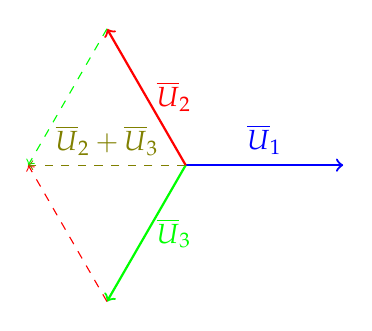
\begin{tikzpicture}
  \draw (0,0) coordinate (N);
  \draw[->, color=blue, thick] (N) -- (0:2) node[above, midway] {$\overline{U}_1$};
  \draw[->, color = red, thick] (N) -- (120:2) node[right, midway] {$\overline{U}_2$};
  \draw[->, color = green, thick] (N) -- (-120:2) node[right, midway] {$\overline{U}_3$};
  % \draw[->, color = red] (N) -- ($(N)!(-120:2)!(0:2)$);%%Projection
  % \draw[->, color = green] (N) -- ($(N)!(120:2)!(0:2)$);%%Projection
  \draw[->, color = green,dashed] (120:2) -- ++(-120:2);
  \draw[->, color = red, dashed] (-120:2) -- ++(120:2);
  \draw[->, color = green!50!red, dashed] (N) -- (-2,0) node[midway, above] {$\overline{U}_2 + \overline{U}_3$};
\end{tikzpicture}
\end{document}